\documentclass[preview]{standalone}
\usepackage{caption}
\usepackage{tikz}
\usetikzlibrary{fit, arrows}
\captionsetup[figure]{labelformat=empty}

\begin{document}
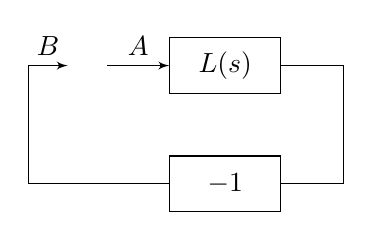
\begin{tikzpicture}[auto, node distance=1.5cm,>=latex']
  \tikzstyle{block} = [draw, rectangle, minimum height=2em, minimum width=4em]
  \tikzstyle{sum} = [draw, fill=white, circle, inner sep=0.5mm]
  \tikzstyle{tmp} = [coordinate]
  \node [tmp] (upperleft) {};
  \node [tmp, right of=upperleft, left=1cm] (outend) {};
  \node [tmp, right of=outend, left=1cm] (input) {};
  \node [block, right of=input] (Ls) {$L(s)$};
  \node [tmp, right of=Ls] (upperright) {};
  \node [block, below of=Ls] (minusone) {$-1$};

  \draw [->] (input) -- node {$A$} (Ls);
  \draw (Ls) -- node {} (upperright) |- node {} (minusone);
  \draw [->] (minusone) -| (upperleft) -- node {$B$} (outend);
\end{tikzpicture}
\end{document}
